%recently finished my uni and get to start choosing where and what I want to do.
%spent a year in japan
%would like to experience more of the world
%want to play in an organisation that has room for growth and the opportunity to effect the way people do things
%


\documentclass[10pt, a4paper]{report}
\usepackage{geometry}                % See geometry.pdf to learn the layout options. There are lots.
\geometry{lmargin=1cm}
\geometry{rmargin=1cm}
\geometry{tmargin=1cm}
\geometry{bmargin=1cm}



\title{Curriculum Vitae}
\author{Bodey Baker}
%\date{}                                           % Activate to display a given date or no date

\parindent 0pt
\parskip 5pt
\pagestyle{empty}

%\usepackage{CJK}
\usepackage{mdwlist}
\usepackage{graphicx}
\usepackage{booktabs}
\usepackage{flafter}  % Don't place floats before their definition
\usepackage{amsmath,amssymb}  % Better maths support & more symbols
\usepackage[utf8]{inputenc} % Any characters can be typed directly from the keyboard, eg éçñ
%\usepackage{geometry} % to change the page dimensions
\usepackage{enumitem}
\setitemize{noitemsep,topsep=0pt,parsep=0pt,partopsep=0pt,leftmargin=1em}

%empty
\newcommand{\teaching}[1]{}
\newcommand{\engineering}[1]{}
\newcommand{\verbose}[1]{}

%teaching resume (needs to be 2 pages)
%\renewcommand{\teaching}[1]{#1}
%\renewcommand{\engineering}[1]{}
%\renewcommand{\verbose}[1]{}

%Engineering CV
\renewcommand{\teaching}[1]{#1}
\renewcommand{\engineering}[1]{#1}
\renewcommand{\verbose}[1]{#1}

\newcommand{\wh}[5]{{\bf{#2 \hfill #1}}
\begin{tabular}{ll}
\parbox[t]{13cm}{#5}
& \parbox[t]{5.3cm}{ \raggedleft{ {#3}\\{#4}\\}}\end{tabular}}

%\newcommand{\sk}[3]{\begin{basedescript}{\desclabelstyle{\pushlabel}\desclabelwidth{10em}}
%\item[#1] #2 \end{basedescript}#3}
\newcommand{\sk}[3]{\subsubsection*{#1} {#2}{#3}}

\newcommand{\pa}[3]{#1 - #2}

\makeatletter\let\MPtrue\@minipagetrue\makeatother

\title{Curriculum Vitae\\~\\of}
\author{Bodey Baker}% \\(?????????)\\ \\}



\begin{document}
%\begin{titlepage} \maketitle \end{titlepage}

%%\section*{Personal details}
%\begin{basedescript}{\desclabelstyle{\pushlabel}\desclabelwidth{8em}}\item[Name] Bodey Royce Baker
%%\item[Home address] 3/28-34 Stirling Hwy.\\ Nedlands, W.A. 6009\\Australia
%%\item[Current mailing address] Bodey Baker\\
%%School of Computer Science \& Software Engineering\\
%%The University of Western Australia\\
%%Crawley, W.A. 6009\\
%%Australia
%\item[Phone] (+61) 420901219   
%\item[Email] bodeybaker@gmail.com
%\item[Date of Birth] 5th October 1984
%\item[Citizenship] Australian
%%\item[Visa] Working Holiday Visa
%%\item[Current Date] \today
%\end{basedescript}

\begin{minipage}{0.82\linewidth}
\begin{tabular}{ll}
{\bf Name} & Bodey Royce Baker \\ 
{\bf Date of Birth} & 5th October 1984 \\
{\bf Citizenship} & Australian \\
{\bf Email} & bodeybaker@gmail.com \\
{\bf Phone} & +82-10-2186-1005 \\
{\bf Location} & Seoul, South Korea \\

\end{tabular}
\end{minipage}
\hfill
\begin{minipage}{0.6\linewidth}
{%
\setlength{\fboxsep}{0pt}%
\setlength{\fboxrule}{1pt}%
%\fbox{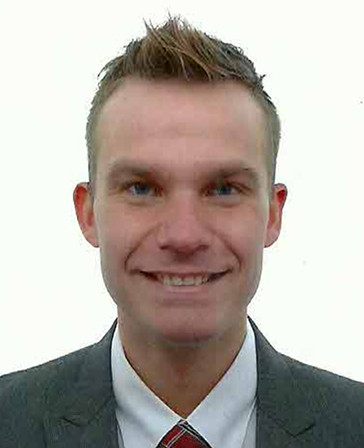
\includegraphics[height=40mm]{pic6.jpg}}%
}%
\end{minipage}

\section*{Skills}

\begin{tabular}{lp{14cm}}
{\bf Languages} & English (Native), Japanese (Basic), Korean (Basic)\\  \addlinespace
{\bf Programming} &  Java, Python, C, JavaScript (Highly Proficient) \\  \addlinespace
{\bf } &  C++, C\#, MATLAB, PHP, xHTML, CSS, MySQL (Proficient) \\  \addlinespace
{\bf Familiar Platforms} & .NET, Gumstix (OMAP3430), Stellaris microcontrollers, Android \\ \addlinespace
{\bf Theory} & Algorithms, Artificial Intelligence (AI), Machine Learning, Multi\-Agent Systems (MAS), Computer Vision, Visualisation, Parallel Computing \\  \addlinespace
%{\bf Visualisation Software} & Amira, Dristi \\  \addlinespace
{\bf Engineering} & Robotics, Embedded Systems \\  \addlinespace
{\bf Mathematics} & Linear Algebra,  Multi-Variable Calculus, Probability \& Statistics, Control Theory \\  
{\bf CAD Software} & Autodesk Inventor, SolidWorks \\  \addlinespace
%{\bf Office Software} & MS Word, \LaTeX , OpenOffice/LibreOffice \\  \addlinespace
{\bf Operating Systems} &  Linux, UNIX, Mac OS X, Windows XP/7/8 \\  \addlinespace
\addlinespace
\end{tabular}

%%\teaching{
%%\sk{Teaching}{}
%%{I have attended the "Seminars, Tutorials and Laboratories" teaching course at the University of Western Australia. Following this I tutored the units ``Modelling and Computing Analysis for Engineers" and ``Mechatronics Systems" for one semester.}
%%\sk{English Ability}{I am a native English speaker from Australia who has completed a computer science bachelors degree with honours and written three scientific papers that have been published.}
%%{}
%%}
%\begin{basedescript}{\desclabelstyle{\pushlabel}\desclabelwidth{12em}}
%\item[Languages] English (Native), Japanese (Basic-Intermediate), Korean (Basic)
%\end{basedescript}
%\engineering{
%%\section*{Computing Skills}
%\begin{basedescript}{\desclabelstyle{\pushlabel}\desclabelwidth{12em}}
%\item[Operating Systems] Linux, UNIX, Mac OS X, Windows XP/7
%\end{basedescript}
%%on vs. in a variety of os's
%%I use and program in a variety of operating systems. At Cyber Technology, most of our programming work is done in linux. Previously I've used OpenEmbedded and Linux From Scratch to compile Linux Systems, and written code for user and kernel space applications. I've also coded applications and dynamic libraries for windows using .NET and my home laptop runs OS X.
%\begin{basedescript}{\desclabelstyle{\pushlabel}\desclabelwidth{12em}}
%\item[Programming] Java, Python, C (Highly Proficient)
%\item[] C++, C\#, MATLAB, PHP, xHTML, CSS (Proficient)
%\end{basedescript}
%%\begin{basedescript}{\desclabelstyle{\pushlabel}\desclabelwidth{12em}}
%%\item[Programming] Java
%%\end{basedescript}
%%The majority of my university projects have been implemented in Java and since working at Cyber Technology I've started using of more advanced language features and design patterns with a large piece of software, their control manger for their UAV systems.
%%\begin{basedescript}{\desclabelstyle{\pushlabel}\desclabelwidth{12em}}
%%\item[] Python
%%\end{basedescript}
%%A data analysis project at JRB Engineering required learning Python and since then it has been used for a variety of quick implementation, testing and analysis tasks both there and at my current position at Cyber Technology.
%%\begin{basedescript}{\desclabelstyle{\pushlabel}\desclabelwidth{12em}}
%%\item[] C, C++, MATLAB
%%\end{basedescript}
%%\indent Much of my work at Cyber Technology has been writing low level code for our peripheral devices in C.  While at MRX I worked on a number of projects using Visual C++. My honours project and my iVEC internship were implemented in C++ and C respectively and both required some analysis in MATLAB.
%%\begin{basedescript}{\desclabelstyle{\pushlabel}\desclabelwidth{12em}}
%%\item[]  PHP, xHTML, CSS
%%\end{basedescript}
%%\indent Over the course of my degree I have designed websites as a means of assessment. I have also been the web-master for the Bantus Capoeira website and been involved with the design, construction and maintenance of the Association of Mechatronic's website.
%%\begin{basedescript}{\desclabelstyle{\pushlabel}\desclabelwidth{12em}}
%%\item[] Bash, Haskell [{\em Previously Used}]
%%\end{basedescript}
%%\indent I have used Bash scripting extensively for a variety of short tasks, but this has not been mastered. Haskell was introduced early in my university career and has not been built upon.
%
%\begin{basedescript}{\desclabelstyle{\pushlabel}\desclabelwidth{12em}}
%\item[Theory] Algorithms, Artificial Intelligence (AI), Machine Learning, Multi\-Agent Systems (MAS),\\ Computer Vision, Visualisation, Parallel Computing
%\end{basedescript}
%
%%\begin{basedescript}{\desclabelstyle{\pushlabel}\desclabelwidth{12em}}
%%\item[Theory] Algorithms
%%\end{basedescript}
%%\indent I've gained  a thorough understanding of algorithm design, speed and memory use through taking units on algorithm design, searching, planning and parallel computing. These skills have been further strengthened by my work at iVEC.
%%\begin{basedescript}{\desclabelstyle{\pushlabel}\desclabelwidth{12em}}
%%\item[] Artificial Intelligence (AI), Multi\-Agent Systems (MAS)
%%\end{basedescript}
%%%My computer science honours project was on team work in robot soccer. This strengthened my understanding of MAS and AI theory, applications and current research.
%%\begin{basedescript}{\desclabelstyle{\pushlabel}\desclabelwidth{12em}}
%%\item[] Computer Vision, Visualisation, Parallel Computing
%%\end{basedescript}
%%%Units in computer vision and visualisation and the iVEC Internship gave me a thorough grounding in these skills.
%\begin{basedescript}{\desclabelstyle{\pushlabel}\desclabelwidth{12em}}
%\item[Familiar Hardware] Cray XT3, AIBO ERS-7, Gumstix (OMAP3430), Stellaris microcontrollers
%\item[CAD Software] Autodesk Inventor, SolidWorks
%\item[Visualisation Software] Amira, Dristi
%\item[Office Software] MS Word, \LaTeX , OpenOffice/LibreOffice
%\item [Engineering] Robotics, Embedded Systems
%\item[Mathematics] Linear Algebra, Statistics, Control Theory
%%\item[Modelling] Dynamic Systems, Static Systems, Electrical Circuits, Vibration
%\end{basedescript}
%}

\section*{Experience}

\wh{July 2010 - July 2012}
{Avionics Software Engineer}
{Cyber Technology}
%{1C Ambitious Link \\Bibra Lake WA 6163 \\ 
{Australia}
{
\begin{itemize}
\item Jointly implemented the ground control manager for configuration and control of unmanned aerial vehicles. This is written in Java Script \& PHP and interfaces with the ground control server across a network.
\item Jointly implemented the JAVA prototype for the ground control manager.
\item Designed and wrote the firmware and boot loaders for our peripheral devices that transcode data from company UDP and CAN protocols to interface with transmitters and other third party devices using C and the Code Sourcery toolchain.
\item Analysis of data/prototyping in Python; Data stream conversion in C\#.
\end{itemize}
%- Skills: Java, C, Python, C\#, MySQL \newline
%- Data Formats: CAN, UDP
}

\wh{May 2009 - June 2010}
{Undergraduate Engineer}
{JRB Engineering}
%{24 Drummond Pl. \\ West Perth WA 6005\\ 
{Australia}
{
\begin{itemize}
\item Processed accelerometer data in Python to ensure vehicles met vibration requirements.
\item Implemented some visualisation software using Visual C\#.
\item Improved the pattern matching algorithm for brake pad detection using Python.
\item Used Visual C++ to remove noise during the post processing of objects in laser scanning data.
\end{itemize}
}

\wh{May 2008 - February 2009}
{Assistant English Teacher}
{W5 Staff Services}
%{Hanaguruma bldg. Kitakan 3F\\ 5-4-14 Meieki, Nakamura-ku\\ Nagoya-shi, Aichi, 
{Japan \\ ~}
{
\begin{itemize}
\item Taught English to primary and junior high school students.
\item Duties: planning lessons; teaching; communicating with students.
\item Skills: teaching; public speaking; motivation of others; integrating into new cultures.
\end{itemize}
}

\engineering{
\wh{January 2008 - March 2008}
{Undergraduate Engineer}
{JRB Engineering}
%{24 Drummond Pl. \\ West Perth WA 6005\\ 
{Australia \\ ~}
{
\begin{itemize}
\item Visualised the output of log files using Visual Studio with C++.
\item Created dynamic libraries for data processing routines in Windows
\item Modelling parts for a road rail vehicle using Autodesk Inventor.
\end{itemize}
 }
 }

\engineering{
\wh{August 2007 - January 2008}
{Research Assistant}
{Centre for Exploration Targeting \\ University of Western Australia}
%{26 Dick Perry Ave. \\ Kensignton WA 6151\\ 
{Australia}
{Studied the feasibility of using Amira to process 3D data sampled from rock samples to analyse their composite structure and visualise the segmented data using a 3D projector for better data exploration.}}

\newpage

\wh{July 2007 - November 2007}
{Tutor}
{University of Western Australia}
%{35 Stirling Hwy.\\ Crawley WA 6009\\ Australia
{~}
{
\begin{itemize}
\item Tutored: Modelling and Computing Analysis for Engineers; \\ Mechatronics Systems; Java.
\item Required a detailed knowledge of MATLAB, LabVIEW and Java.
\item Duties: teaching, lab demonstrating and marking.
\end{itemize}
}

\wh{March 2007 - December 2007}
{Research Assistant}
{Centre for Exploration Targeting \\ University of Western Australia}
%{35 Stirling Hwy.\\ Crawley WA 6009\\ Australia
{~\\~}
{
\begin{itemize}
\item Analysed the directional variation of roughness across a rock surface.
\item Continuing from iVEC work and Eventuating in a paper.
\end{itemize}
}

\wh{December 2006 - March 2007}
{iVEC Intern}
{Centre for Exploration Targeting \\ University of Western Australia}
%{35 Stirling Hwy.\\ Crawley WA 6009\\ Australia
{~\\~}
{
\begin{itemize}
\item Researched an algorithm to analyse the directional variation of roughness of a rock surface from 3D geometric data using MPI for C.
\item Skills Gained: visualisation; parallel computing; algorithm design.
\end{itemize}
}
%\wh{2004 - 2006}
%{Clerk}
%{Mothers Foods}
%{Nedlands WA\\ Australia}
%{I worked as a clerk within a pressured time constrained environment with responsibilities including closing the store and handling money.}
\section*{Education}

\subsection*{Bachelor of Engineering}
	\begin{basedescript}{\desclabelstyle{\pushlabel}\desclabelwidth{11em}}
	%\item[Started]  2003
	\item[Completed] 2011
	%\item[GPA (WAM)] 3.977 (57.791)
	\item[Institution] The University of Western Australia
	\item[Majors] Mechatronics
	\item[Mechatronics Thesis] {\em Developing a stand alone wireless sensor network for damage detection using the impedance method}
	\end{basedescript}
This project required changing the platform of an active damage detection system from large and expensive laboratory equipment to a cheaper and smaller embedded platform that is more applicable to the field. This involved cross-compiling for an embedded platform using OpenEmbedded, user and kernel level code, some circuit design and mathematical analysis of sensor readings.

{\bf Developed Skills:} Cross-compiling; embedded software; kernel level development; linux architecture; C; Python; hardware; OpenEmbedded; SPI; LabVIEW; Networks.
	\engineering{
	\begin{basedescript}{\desclabelstyle{\pushlabel}\desclabelwidth{5em}}
	\item[Units:] 

% \begin{description*}{\desclabelstyle{\pushlabel}\desclabelwidth{5em}}
\begin{tabular}[h]{lr}
{\bf Algorithms for AI} & Distinction\\
{\bf Embedded Systems} & Distinction\\
{\bf Algorithms} & Distinction\\
{\bf C Programming} & Distinction\\
{\bf Foundations of Computer Science} & Distinction\\
{\bf Robotics and Automation} & Credit\\
{\bf Real-time Distributed Computer Systems} & Credit\\
{\bf Concurrent Programming} & Credit\\
{\bf Computer Architecture} & Credit\\
{\bf Operation Systems} & Credit\\
{\bf Professional Computing} & Credit\\
{\bf Mechatronics Systems} & Credit\\
{\bf Advanced Control Engineering} & Credit\\
{\bf Control and Mechatronics} & Credit\\
{\bf Manufacturing} & Credit\\
{\bf Software Engineering Design} & Credit\\
{\bf Engineering Dynamics} & Credit\\
% {\bf Engineering Design} & Pass
{\bf Intro Elec. Eng.} & Credit\\
{\bf Intro Mech. Eng.} & Credit\\
{\bf Software Engineering 104} & Credit\\
% {\bf Computer Engineering} & Pass
% {\bf Intro. Prof. Eng.} & Pass
{\bf Object Oriented Programming} & Credit \\
% {\bf Data Structures \& Algorithms} & Pass
% {\bf foundations of IT} & Pass
% {\bf Java Programming} & Pass
% {\bf Mathematics 132} & Pass
% {\bf Mathematics 101} & Pass
% {\bf Mathematics 101} & Pass
% {\bf Physics 100} & Pass
\end{tabular}
	\end{basedescript}
	}


\subsection*{Computer Science with Honours} % Honours (2A)
	\begin{basedescript}{\desclabelstyle{\pushlabel}\desclabelwidth{11em}}
	\item[Completed] 2006
	\item[Institution] The University of Western Australia
	\item[GPA (WAM)] 6.00 (74.13)
	\item[Thesis] {\em Strategy specification for teamwork in robot soccer}
\end{basedescript}
Researched planning in multi-agent systems where a team of agents have a common goal, are being hindered by other agents, only have a limited view of the world, and due to time constraints not all team members can be informed of the planned solution but they must still co-ordinate in a reasonable manner.

{\bf Developed Skills:} Algorithms; C++; Visual Studio.
%Must write about the thesis here
\begin{basedescript}{\desclabelstyle{\pushlabel}\desclabelwidth{5em}}
\item[Units:]

% \begin{description*}{\desclabelstyle{\pushlabel}\desclabelwidth{5em}}
\begin{tabular}[h]{lr}
{\bf Computer Vision} & High Distinction\\
{\bf Scientific Communication} & High Distinction\\
{\bf Visualisation} & High Distinction\\
\end{tabular}
\end{basedescript}

\subsection*{Secondary Education}
	\begin{basedescript}{\desclabelstyle{\pushlabel}\desclabelwidth{13em}}
	\item[1999-2001] Manjimup Senior High School
	\item[TER] 95.55 percentile
	\item[TEE subjects] Calculus, Applicable Mathematics, Physics, Chemistry, \\ Geography, English
	\end{basedescript}


\section*{Scholarships and Prizes}
{\bf 2007:} Top of the Computer Science honours unit ``Scientific Communication" \newline
{\bf 2006:} Commonwealth Accommodation Scholarship \newline
{\bf 2001:} Institute of Engineers award for attaining a TEE score above 75\% in:\\
 Chemistry, Physics, Calculus and Applicable Mathematics. \newline
{\bf 2000:} Olympic Torch Escort Runner	 \newline
{\bf 2000:} Australian Mathematics Competition High Distinction \newline
{\bf 1996:} Citizenship Award

% \section*{Professional Experience}
% \subsection*{Courses taught}
% \subsection*{Theses supervised}

\section*{Publications}
B. Baker, K. Gessner, E.J. Holden, and A. Squelch,  \emph{Automatic detection of anisotropic features on
rock surfaces}, Geosphere, Geological Society of America, (April 2008), 4(2):418-428\\
\\
B. Baker, M. Reynolds and W. Liu, \emph{Strategy specification for
  teamwork in robot soccer}, PCAR '06: Proceedings of the 2006 international
  symposium on Practical cognitive agents and robots (New York, NY, USA), ACM
  Press, 2006, pp.~129--140.\\
  \\
B. Baker, K. Gessner, E.J. Holden, and A. Squelch, \emph{Automatic analysis and 
visualisation of rock surface roughness,} Deformation in the desert (Alice Sprints, Northern 
Territory, Australia), Tectonics \& Structural Geology, Geological Society of Australia, July 
2007

%\nocite{*}
%~\cite{baker06strategy,baker07automatic}
%\bibliography{mine}

% \section*{Grants}

\section*{Professional affiliations}
Webmaster of Ancestrais Capoeira (2007-2008) \newline
President of the UWA Association of Mechatronics Engineers (2007) \newline
Social Engineer of the UWA Association of Mechatronics Engineers (2006) \newline
Vice-President of the UWA Computer Science Students Club (2006) \newline
Ordinary Committee Member in the UWA Computer Science Students Club (2005) \newline

% \section*{Volunteer Activities}
\section*{Interests}
{\large Soccer, Martial Arts, Rock Climbing, Capoeira, Open Source Software, Machine Learning, Space, Translation, Snow Boarding, Linux, Android, Travelling, Languages, Cultures.}

\pagebreak

\section*{Quotations}
{\large ``Bodey worked very hard and long hours during his time at Cyber Technology. He assisted the CyberPilot Project by being innovative and thorough. His ability to plan and develop key process improvements has resulted in outcomes well ahead of expectations and lead times.
\\
\\
I would recommend Bodey to anyone seeking a reliable, efficient and well informed engineer and team leader.''}

~\hspace*{4em} {\bf Paul G. Dewar} - {\em Chief Operating Officer - Cyber Technology}

\vspace{1em}

\hfill {\large ``Bodey's performance at the company was outstanding. He was on time, showed initiative, worked hard and was highly productive. I highly recommend him for research 
and development engineering work.''}

\hfill {\bf Xavier Orr} - {\em Director of Research and Development - Cyber Technology} \newline
%\begin{tabular}[h*]{lcr}
%\parbox{5cm}{{\bf Jim Blair}\\ Managing Director\\ JRB Engineering\\ West Perth WA\\  +61 4 1904 1710\\ JimBlair@jrbeng.com.au} &
%\parbox{5cm}{{\bf Dr Klaus Gessner}\\ Senior Lecturer\\ University of WA\\ Crawley WA\\ +61 8  6488 7148 \\ kgessner@cyllene.uwa.edu.au}&
%\parbox{5cm}{{\bf Dr Mark Reynolds}\\Associate Professor\\ University of WA\\ Crawley WA\\ +61 8 6488 2279 \\ mark@csse.uwa.edu.au}
%\end{tabular}

\pagebreak

\setlength{\topmargin}{-1.5in}
\setlength{\oddsidemargin}{-1in}

%\begin{figure}[h!]
%   \centering
%   
\includegraphics[height=1.08\vsize]{a_deg_me.jpg} 
%\end{figure}
%
%\begin{figure}[h!]
%   \centering
%   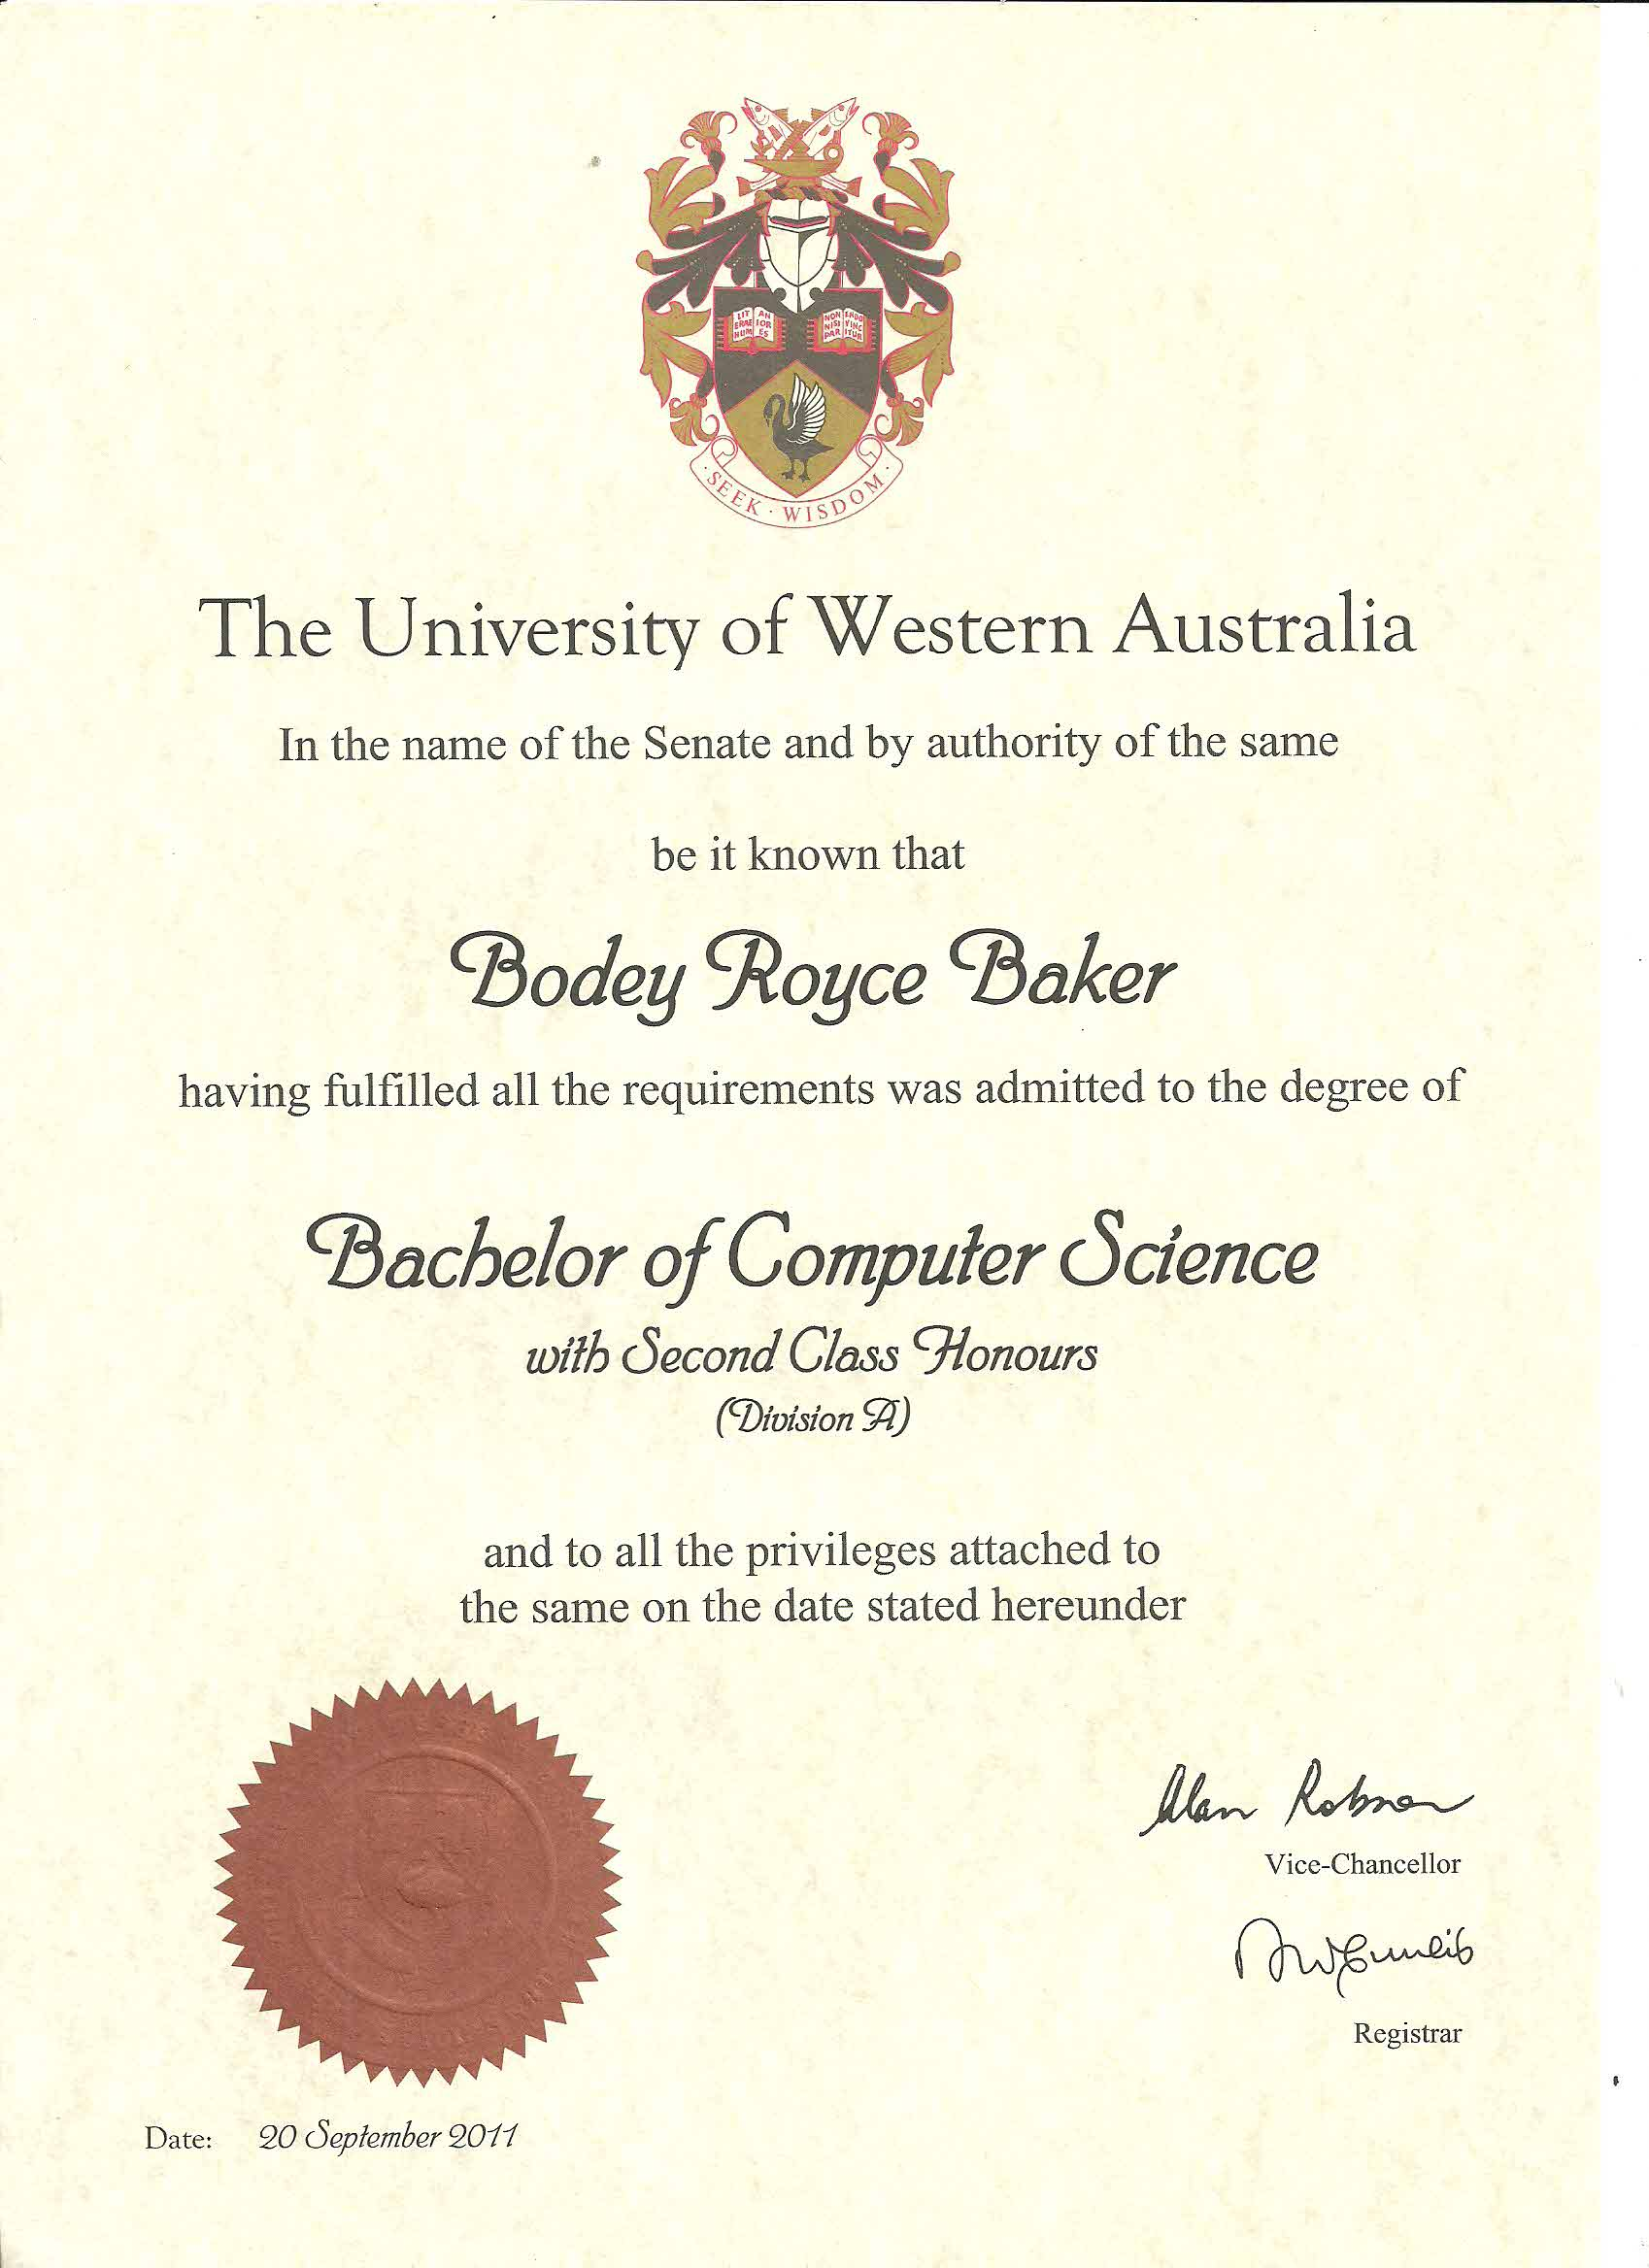
\includegraphics[height=1.08\vsize]{a_deg_cs_honours.jpg} 
%\end{figure}
\begin{figure}[h!]
   \centering
   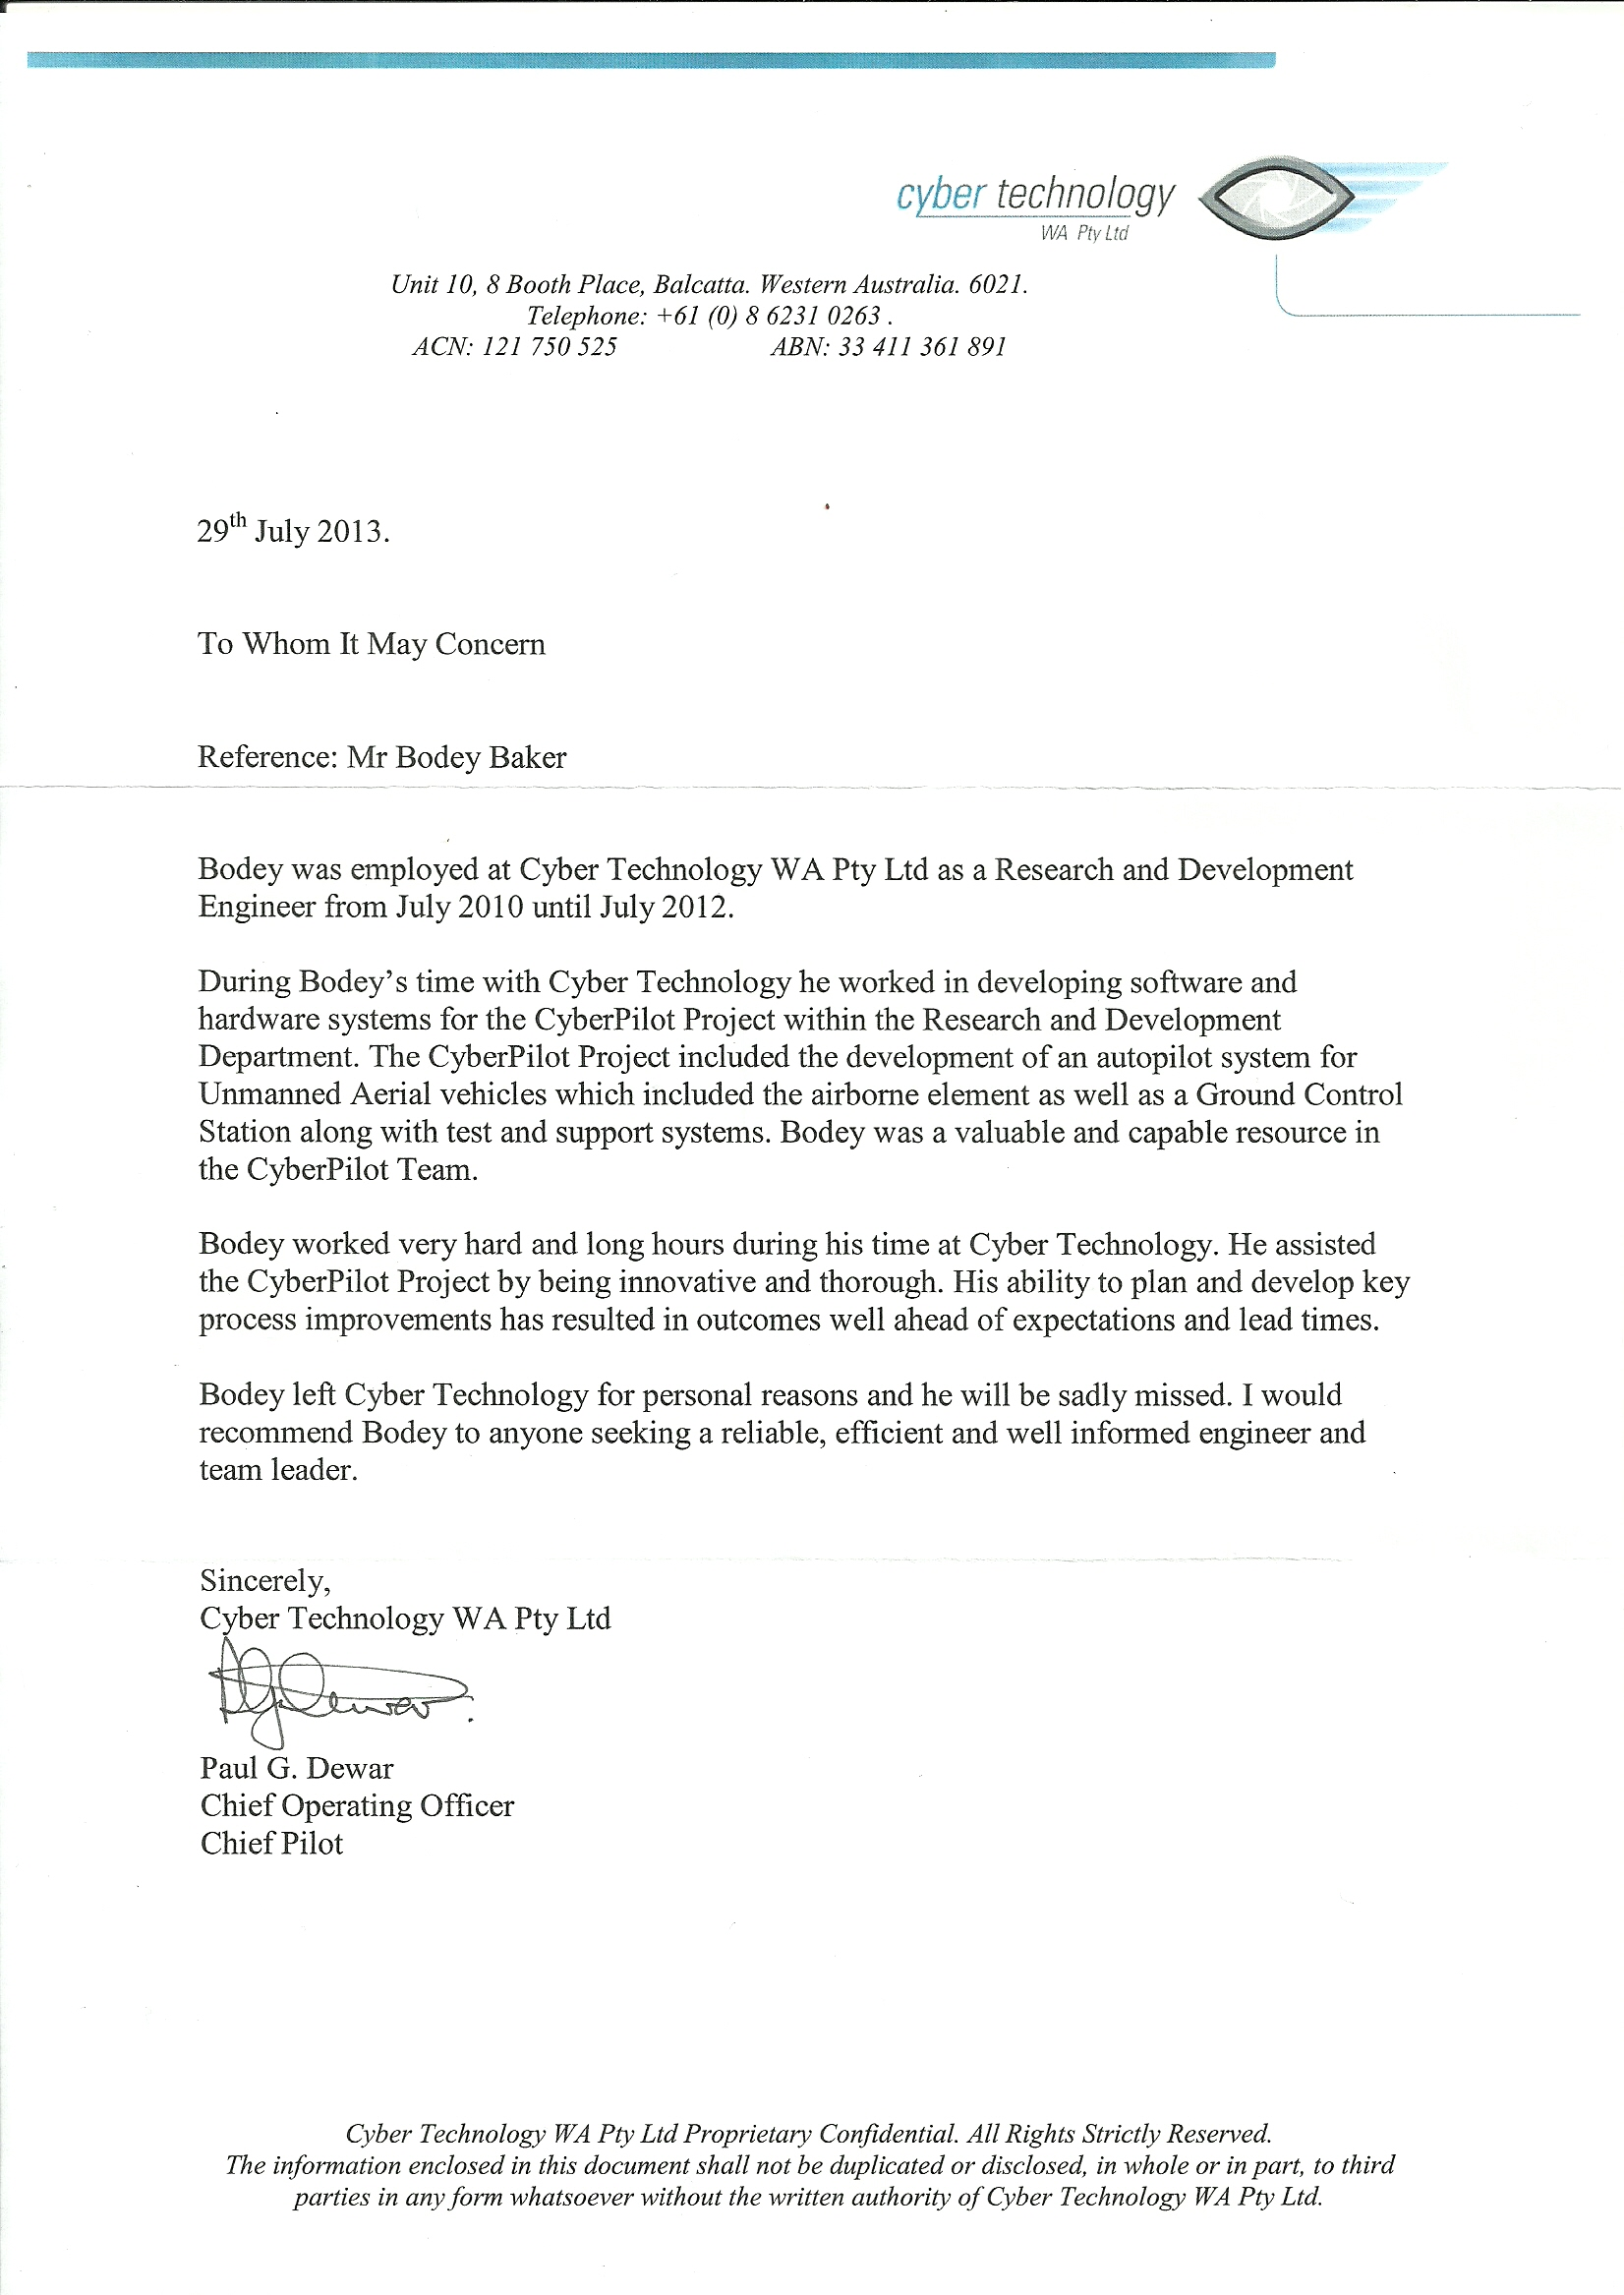
\includegraphics[height=1.08\vsize]{images/ref-paul.jpg} 
\end{figure}


\end{document}